\documentclass{article}
\usepackage{ctex}

\usepackage[letterpaper,top=2cm,bottom=2cm,left=3cm,right=3cm,marginparwidth=1.75cm]{geometry}

\usepackage{amsmath}
\usepackage{graphicx}
\usepackage[colorlinks=true, allcolors=black]{hyperref}
\usepackage{booktabs}
\usepackage{tabularx}
\usepackage{array}
\usepackage{enumitem}
\usepackage{float}
\usepackage{longtable}
\usepackage{array}
\usepackage[numbers]{natbib}
\usepackage{tikz}
\usetikzlibrary{arrows.meta, positioning, shapes.geometric, fit, calc}
\newcommand{\upcite}[1]{\textsuperscript{[\citenum{#1}]}}

% 表格辅助
\newcolumntype{Y}{>{\raggedright\arraybackslash}X}
\newcolumntype{C}[1]{>{\centering\arraybackslash}m{#1}}

\begin{document}

\begin{center}
    \vspace*{1em}
    {\huge \bfseries \heiti 死亡游戏中的非合作博弈与信任机制：以《弥留之国的爱丽丝》红心7与红心J为例}
    \vspace{1.5em}
\end{center}

\begin{abstract}
近年来，影视文本逐渐成为博弈论教学与社会科学分析中的重要案例来源。与传统数学化模型相比，影视叙事能够通过具体人物、极端情境与可观察行为呈现战略互动的过程，使“玩家”“策略”“收益”“信息”与“均衡”等概念具有更直观的解释空间。本文以《弥留之国的爱丽丝》中的红心7“狼与羊”与红心J“单人牢房”为研究对象，尝试将死亡游戏中的剧情冲突转化为博弈论模型，分析极端生存情境下个体理性、信任机制与非合作行为之间的关系。
（以上表述表现出环境的高度限制，质疑了其现实场景的意义，改成在极端情境下人的理性和本能充分激发，博弈更纯粹之类的说法）

本文借鉴影视博弈分析中的场景化处理方法，将剧情拆解为若干关键决策节点，并依次识别其中的玩家、可选策略、收益结构与可能均衡。红心7中，游戏规则规定最终只有“狼”能够存活，其他“羊”则面临死亡，由此形成高度零和的生存竞争结构。本文将其视为一个由熟人关系嵌入零和规则后的非合作博弈，重点讨论友情承诺为何难以稳定、个体理性为何会压倒集体最优，以及牺牲行为如何体现收益函数的变化。红心J中，玩家无法观察自身花色，只能依赖他人提供信息，同时隐藏身份的红心J具有操控信息与破坏信任的动机。本文将其视为信息不对称条件下的动态信任博弈，重点分析信号传递、重复互动、联盟形成与贝叶斯式信念更新在玩家选择中的作用。

研究认为，红心7与红心J之间存在明显的理论递进关系：前者呈现的是零和生存规则对熟人信任的瓦解，后者则进一步展示信息不对称环境中陌生人信任机制的生成、利用与崩塌。二者共同说明，《弥留之国的爱丽丝》中的红心游戏并非单纯依靠残酷剧情制造冲突，而是通过规则设计改变玩家的收益结构，使合作、背叛、牺牲与验证均成为特定制度环境下的理性选择。通过对关键节点的模型化与 if 线推演，本文旨在说明人物并非没有行动选项，而是在既定规则、信息限制与收益压力下，难以找到同时满足生存、合作与稳定的最优路径。

\textbf{关键词：}《弥留之国的爱丽丝》；非合作博弈；零和博弈；信息不对称；信任机制；纳什均衡
\end{abstract}

\section{引言}

博弈论关注的是多个决策主体在相互影响条件下如何作出选择的问题。与单个个体的孤立决策不同，博弈论强调个体行为的结果不仅取决于自身策略，也取决于其他参与者的策略选择。因此，在博弈论分析中，“玩家”“策略”“收益”“信息结构”与“均衡”构成了理解战略互动的基本要素。无论是市场竞争、政治谈判、社会合作，还是日常生活中的信任与背叛，只要一个人的选择会受到他人选择的影响，就可以被纳入博弈论的分析框架之中。

近年来，流行影视作品也被用于解释经济学和博弈论概念。相较于抽象公式和纯理论模型，影视文本具有情境具体、冲突集中、人物行为可观察等特点，能够将复杂的战略互动转化为更直观的案例。已有研究表明，以影视场景辅助博弈论教学，有助于学习者从具体情境中理解玩家、策略、收益和均衡等核心概念\upcite{geerling2023squidgame}。本文在此基础上进一步关注影视剧情的模型化分析，即如何将死亡游戏中的规则、人物和行为转化为可讨论的博弈结构。

\begin{figure}[H]
    \centering
    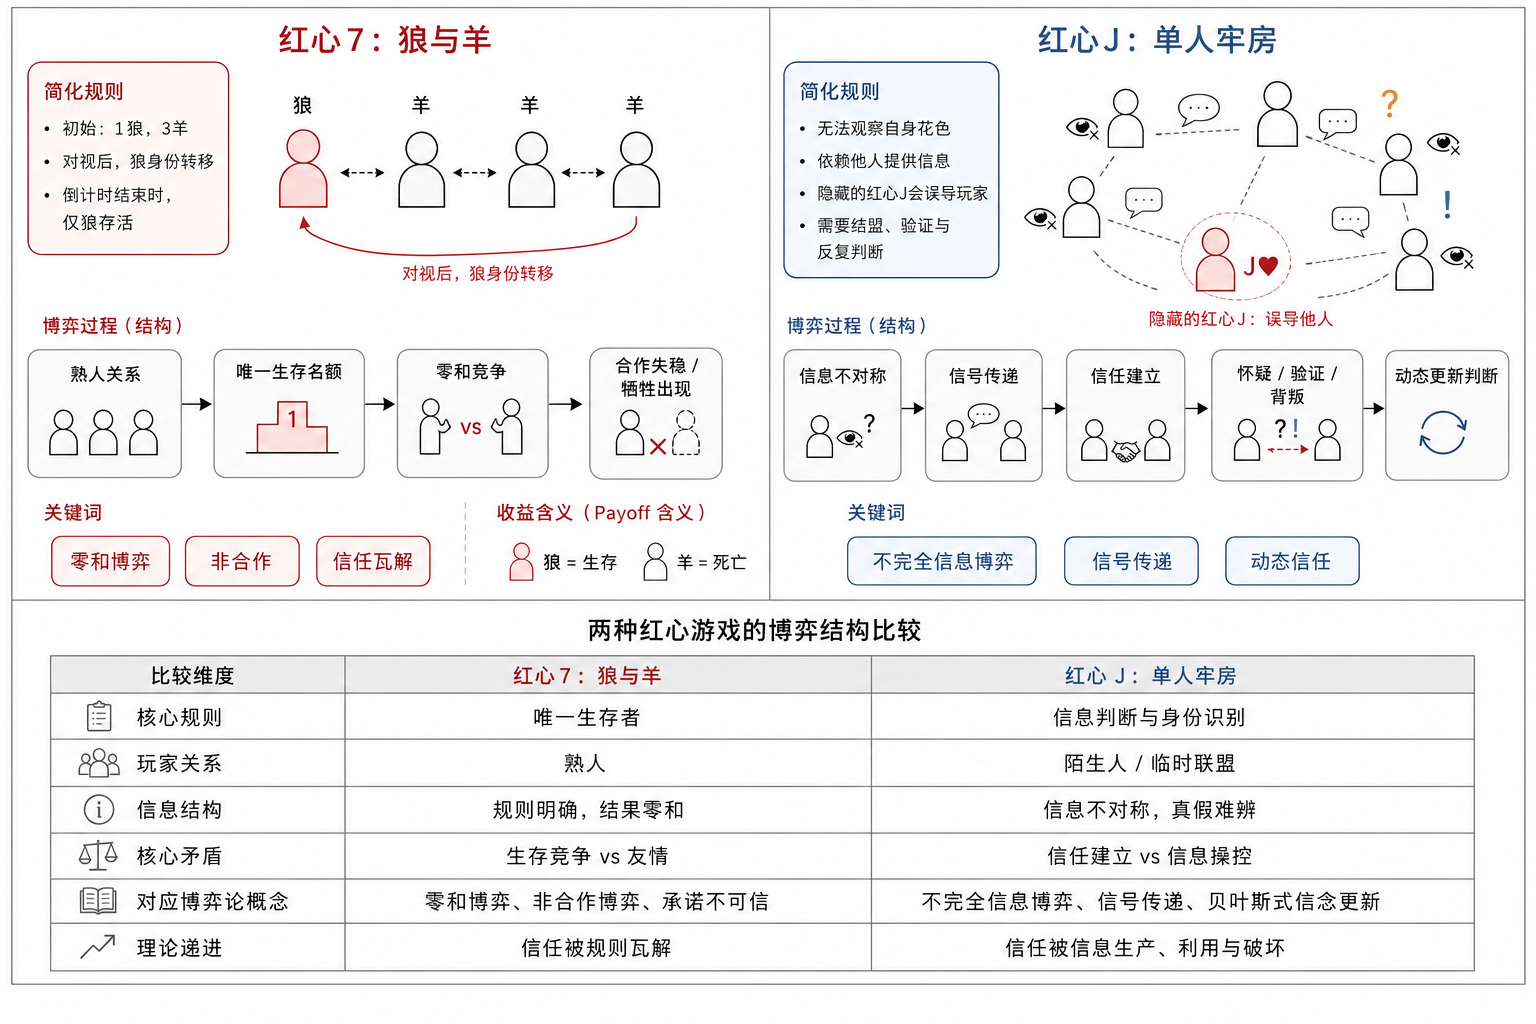
\includegraphics[width=1\textwidth]{./fig/游戏规则.png}
    \caption{红心7与红心J的规则结构及博弈特征比较}
    \label{fig:gameRule}
\end{figure}

基于这一方法，本文选择《弥留之国的爱丽丝》中的红心7“狼与羊”和红心J“单人牢房”作为研究案例。之所以选择这两个游戏，是因为它们同属于红心类型，均以心理压力、信任关系和背叛风险为核心，但二者的博弈结构又具有明显差异。红心7发生在较小规模的熟人群体之中，主要矛盾是唯一生存名额与既有情感关系之间的冲突；红心J则发生在较大规模的陌生人群体之中，核心矛盾是信息不对称条件下真实信息的获取、验证与操控。前者更适合用于分析零和博弈、不可信承诺和个体理性与集体理性的冲突，后者则更适合用于分析信号传递、重复博弈、联盟形成和信念更新。二者结合，能够形成从“生存名额竞争”到“信息信任竞争”的理论递进。如图~\ref{fig:gameRule} 所示中解释了两种游戏的具体规则以及博弈结构的比较。

在红心7中，玩家被分为“狼”与“羊”。游戏结束时，只有狼能够存活，羊则会死亡。这一规则使得玩家之间的关系被直接改造为零和关系，即一名玩家的生存往往意味着其他玩家的死亡。在这种结构下，即便玩家之间原本存在友情、信任或道德承诺，这些关系也会受到生存收益的强烈冲击。本文关注的问题并不是简单判断人物是否自私或是否善良，而是分析在规则规定“只能有一人存活”的前提下，为什么合作承诺难以成为稳定均衡，为什么抽签、轮流、口头让渡等看似公平的方案缺乏执行力，以及为什么最后的牺牲行为需要通过收益函数变化而非普通理性选择来解释。

与红心7相比，红心J的复杂性主要来自信息结构。玩家无法看到自己项圈后的花色，只能依靠他人告知。与此同时，隐藏在玩家中的红心J具有误导他人、制造不信任并延长自身生存的动机。因此，红心J并不是简单的猜测游戏，而是一个围绕信息真实性展开的动态博弈。玩家必须不断判断他人提供的信息是否可信，也必须通过结盟、观察、交叉验证和试探来降低被欺骗的风险。在这一过程中，完全信任会使玩家容易被操控，完全不信任又会导致信息断裂和生存风险上升。因此，红心J为分析“有限信任”“声誉机制”和“贝叶斯式信念更新”提供了较为典型的叙事场景。

本文的研究目标并不是证明影视作品完全符合标准博弈论模型。相反，影视作品作为叙事文本，往往包含情感、偶然性、人物成长和戏剧化处理，其复杂程度不可能被单一模型完全覆盖。因此，本文采用的是一种“模型化解释”而非“完全形式化证明”的路径。首先提取游戏规则中与战略互动有关的部分，其次识别关键决策节点，再将人物转换为玩家，将行为转换为策略，将剧情结果转换为收益结构，最后结合得益矩阵、均衡分析和 if 线推演解释人物选择的合理性与局限性。换言之，本文关注的是，在给定规则和信息条件下，人物为什么会作出某种选择；如果他们选择另一种策略，结果是否会发生改变；以及这些选择是否能够构成稳定均衡。

围绕上述问题，本文将按照以下结构展开。第一部分介绍影视文本与博弈论分析之间的关系，并说明本文的案例选择与分析方法。第二部分分析红心7“狼与羊”的规则结构，将其建模为零和生存博弈，讨论熟人关系在极端非合作规则下的瓦解机制。第三部分分析红心J“单人牢房”的信息结构，将其建模为信息不对称条件下的动态信任博弈，讨论玩家如何在信任、验证和背叛之间进行策略选择。第四部分进一步比较两个游戏的理论递进关系，并通过 if 线推演说明不同策略组合可能导致的结果变化。最后，本文总结《弥留之国的爱丽丝》红心游戏对理解非合作博弈与信任机制的启示。

基于上述问题，本文将依次分析红心7与红心J的博弈结构，并进一步比较二者在收益冲突、信息不对称与信任机制上的递进关系。

\section{文献与理论基础}

\subsection{影视文本与博弈论分析}

博弈论本身具有较强的抽象性，初学者往往需要在玩家、策略、收益和均衡之间建立较高程度的形式化理解。如果只依赖公式推导和概念说明，学生容易将博弈论理解为脱离现实情境的数学工具，而难以意识到战略互动广泛存在于社会关系、组织决策和日常选择之中。Dixit\upcite{dixit2005restoring}较早提出，博弈论教学可以通过更具趣味性和现实感的材料展开，以降低概念理解门槛，并帮助学习者从具体情境中把握策略互动的基本逻辑。

已有影视博弈研究的主要价值，不在于把影视作品作为理论的简单例证，而在于提供了一种将叙事情境转化为分析单元的方法。Geerling 等\upcite{geerling2023squidgame}对《鱿鱼游戏》的处理并非按照剧情顺序展开，而是选取若干具有明确策略冲突的片段，将其组织为可讨论的教学场景。这种写法提示本文，在分析《弥留之国的爱丽丝》时，应避免将红心游戏处理成单纯的剧情复述，而应优先识别规则变化、信息差异和策略冲突所形成的决策节点。

因此，本文并不将《弥留之国的爱丽丝》作为单纯的故事文本来讨论，而是将其中的红心游戏视为一种经过叙事包装的战略互动场景。红心7与红心J都以死亡惩罚为背景，但真正值得分析的并不只是死亡本身，而是规则如何改变玩家之间的收益关系，信息如何影响玩家的判断，信任如何被建立、利用和瓦解。本文借鉴影视博弈分析的处理方式，先从游戏规则出发，再抽取关键决策节点，最后将人物行为转化为策略选择，并讨论不同策略组合下的结果与均衡。

\subsection{非合作博弈与零和生存结构}

非合作博弈关注的是没有外部强制契约约束时，理性玩家如何在相互影响的条件下进行策略选择。Osborne 和 Rubinstein\upcite{osborne1994course}将博弈论视为研究互动决策的理论工具，其中玩家的收益不仅取决于自身行动，也取决于其他玩家的行动。Gibbons\upcite{gibbons1992primer}也强调，博弈论的核心问题在于把现实中的互动情境转化为可分析的玩家集合、策略集合和收益函数。对于本文而言，这意味着红心游戏中的人物不应只被理解为剧情角色，而应进一步被抽象为具有目标、约束和策略空间的玩家。

红心7“狼与羊”最突出的结构特征是唯一生存名额。游戏规则规定倒计时结束时只有狼能够存活，羊则会死亡。由于一名玩家获得生存资格往往意味着其他玩家失去生存资格，该游戏呈现出接近零和博弈的收益结构。在零和博弈中，一方收益的增加通常对应另一方收益的减少。虽然红心7中的人物关系包含友情、愧疚和牺牲等非物质因素，但在基本规则层面，生存名额的唯一性使玩家之间首先被推入竞争关系。

这一结构也解释了为什么红心7中的合作承诺很难稳定。若玩家仅以生存作为最高收益，则争夺狼身份具有明显诱因。即便玩家之间口头约定抽签、轮流或让某一人存活，只要规则允许身份在最后阶段通过对视发生转移，失败者就仍然存在偏离协议的动机。由此可见，红心7的悲剧并不只是人物缺乏信任造成的，而是规则本身削弱了承诺的可信性。所谓友情的瓦解，实质上是既有情感关系被嵌入零和收益结构之后产生的策略结果。

纳什均衡概念可以进一步解释这种稳定性问题。纳什均衡强调在给定他人策略的情况下，每个玩家都没有单方面改变策略以提高自身收益的动机。对于红心7而言，单纯的合作或口头承诺难以构成稳定均衡，因为任何处于死亡风险中的玩家都可能通过争夺狼身份改善自身结果。只有当玩家的收益函数发生变化，将朋友生存、道德责任或自我牺牲意义纳入自身收益时，放弃生存机会才可能获得解释。因此，红心7中的牺牲行为不能简单理解为标准理性选择，而应理解为人物偏好结构变化后的特殊选择。

\subsection{信息不对称与信任机制}

与红心7相比，红心J“单人牢房”的核心问题并不是唯一生存名额，而是信息不对称。Akerlof\upcite{akerlof1970lemons}在“柠檬市场”研究中指出，当交易双方掌握的信息不一致时，市场结果可能受到严重影响。虽然该理论最初用于解释二手车市场中的质量不确定性，但其核心逻辑同样适用于红心J的情境。玩家无法观察自己的花色，只能依赖他人告知，因此他人掌握了关于自身生死的重要信息。信息不对称使玩家必须在信任与怀疑之间不断权衡。

Harsanyi\upcite{harsanyi1967games}关于不完全信息博弈的研究为红心J提供了进一步解释。在不完全信息博弈中，玩家无法完全知道其他玩家的类型、偏好或信息状态，只能基于有限信息形成主观判断。红心J中的普通玩家并不知道谁是隐藏的红心J，也无法确认他人提供的信息是否真实。因此，每一次报花色、结盟、试探和背叛都不仅是单次行动，也是对他人类型的判断过程。玩家需要根据他人的历史行为、语言表达、联盟关系和异常举动不断更新信念。

信号传递理论也可以用于解释红心J中的互动结构。Spence\upcite{spence1973job}提出，信息较多的一方可以通过信号影响信息较少一方的判断。在红心J中，告知他人花色本身就是一种信号。真实信号可以帮助他人生存，虚假信号则可能导致他人死亡。由于红心J具有隐藏身份和误导他人的动机，玩家不能仅凭一次信息判断对方是否可信，而需要观察信号在重复互动中的稳定性。由此，信任并不是天然存在的道德关系，而是在多轮互动中通过行为记录、声誉积累和交叉验证逐渐形成的策略资源。

红心J也体现出重复博弈中的声誉机制。玩家在每一轮中的行为会影响他人在下一轮对其可信度的判断。若某一玩家持续提供正确信息，其声誉会提高，更容易获得他人合作。若某一玩家出现说谎、诱导或选择性告知，其声誉会下降，并可能被其他玩家孤立或反制。然而，红心J的特殊性在于，隐藏敌人可能故意在前期提供真实信息来建立声誉，再在关键时刻释放虚假信号。这使得完全信任并不安全，完全不信任也不可行。相对稳定的策略不是无条件相信某个人，而是建立有限信任，并通过多人交叉验证降低被单一信号误导的风险。

\subsection{本文的理论整合思路}

基于上述理论，本文将红心7与红心J分别放在收益结构和信息结构两个层面进行分析。红心7侧重考察唯一生存名额如何影响玩家之间的承诺稳定性，红心J侧重考察信息不对称如何影响玩家之间的信任判断。

在具体分析路径上，本文采用规则识别、节点拆解、模型转化、均衡解释和 if 线推演的方式展开。后文将直接进入两个红心游戏的具体分析。

\section{红心7“狼与羊”的非合作博弈分析}

\subsection{规则结构与玩家转换}

红心7“狼与羊”是《弥留之国的爱丽丝》中最能体现零和生存困境的红心游戏之一。该游戏的核心规则可以概括为，初始状态下有一名玩家为“狼”，其余玩家为“羊”。当狼与羊发生对视后，狼的身份会转移给被对视的羊。倒计时结束时，只有最终处于狼身份的玩家能够存活，其余羊身份玩家则会死亡。由此可见，该游戏并不只是单纯的追逐或躲避游戏，而是通过“唯一生存者”的规则设置，将所有玩家推入高度冲突的生存竞争之中。

从博弈论角度看，红心7的关键不在于人物之间是否存在友情，而在于规则如何改变玩家之间的收益关系。游戏开始前，有栖、苅部、张太等人之间存在较强的熟人关系和情感纽带。然而，在游戏规则公布之后，这种熟人关系被嵌入一个接近零和的收益结构之中。若某一玩家最终成为狼，该玩家获得生存收益，而其他玩家则承担死亡损失。换言之，玩家之间原本可以依靠友情维系的合作关系，被游戏规则重新定义为围绕唯一生存名额展开的策略竞争。

在正式分析中，本文将红心7中的主要人物抽象为理性玩家，将其行为选择转化为策略集合。需要说明的是，这里的“理性”并不意味着人物一定冷酷或自私，而是指玩家会在给定规则、时间压力和信息条件下，根据自身偏好选择相对有利的行动。博弈论中的玩家、策略和收益并不是对人物性格的道德评价，而是对其所处决策结构的形式化表达\upcite{osborne1994course,gibbons1992primer}。

\begin{table}[H]
\centering
\caption{红心7“狼与羊”的玩家、策略与收益结构}
\label{tab:heart7_elements}
\renewcommand{\arraystretch}{1.35}
\begin{tabularx}{\textwidth}{C{3cm}Y}
\toprule
分析维度 & 内容说明 \\
\midrule
玩家 & 有栖、苅部、张太、紫吹等参与者均可视为游戏中的玩家 \\
策略 & 争夺狼身份、逃避对视、寻找他人、隐藏自身、口头承诺、主动牺牲 \\
核心收益 & 最终成为狼意味着生存，最终成为羊意味着死亡 \\
信息条件 & 玩家知道基本规则，也知道狼身份可以通过对视发生转移 \\
关系基础 & 玩家之间存在熟人关系和情感纽带，但规则削弱了承诺的稳定性 \\
博弈类型 & 接近零和博弈的非合作生存博弈 \\
主要矛盾 & 生存竞争与友情承诺之间的冲突 \\
\bottomrule
\end{tabularx}
\end{table}

表~\ref{tab:heart7_elements} 表明，红心7的规则结构具有明显的非合作特征。虽然玩家之间可以进行交流，也可以尝试建立承诺，但游戏并没有提供任何外部执行机制来保证承诺不会被违背。尤其是在倒计时接近结束时，任何仍处于羊身份的玩家都面临死亡压力，因此其偏离原有承诺并重新争夺狼身份的动机会显著增强。这也是红心7区别于一般合作游戏的重要之处。合作并非完全不可能，但合作很难稳定。

\subsection{关键决策节点}

为了避免将红心7分析写成单纯剧情复述，本文将该游戏拆解为若干关键决策节点。每个节点都对应一个具体的策略问题。玩家并不是在抽象地面对“生存还是死亡”，而是在不同时间点上不断面对更具体的选择，例如是否争夺狼身份，是否相信朋友承诺，是否接受抽签安排，是否主动牺牲，以及是否继续寻找其他玩家。

\begin{table}[H]
\centering
\caption{红心7“狼与羊”的关键决策节点}
\label{tab:heart7_nodes}
\renewcommand{\arraystretch}{1.35}
\begin{tabularx}{\textwidth}{C{2.7cm}Y Y Y}
\toprule
决策节点 & 具体问题 & 可选策略 & 对应博弈概念 \\
\midrule
规则公布后 & 玩家如何理解唯一生存名额 & 争夺狼身份或暂时观望 & 零和博弈，非合作博弈 \\
身份转移阶段 & 玩家是否主动制造对视 & 主动追逐，逃避对视，隐藏自身 & 策略互动，收益冲突 \\
口头承诺阶段 & 玩家是否相信朋友承诺 & 接受承诺，怀疑承诺，重新竞争 & 承诺可信性，背叛风险 \\
倒计时后期 & 玩家是否继续争夺狼身份 & 最后争夺，放弃争夺，主动牺牲 & 纳什均衡，偏好变化 \\
结局前选择 & 个体生存是否仍是最高收益 & 保全自身，成全他人 & 利他偏好，非标准收益函数 \\
\bottomrule
\end{tabularx}
\end{table}

分析表~\ref{tab:heart7_nodes} 可得到，红心7的剧情推进可以被转化为一组连续的策略选择。前期玩家可能仍然保留合作幻想，但随着倒计时推进，游戏结构中的零和特征不断强化。此时，玩家对他人承诺的信任程度会下降，个体生存收益会被放大，合作关系也更容易被重新解释为策略风险。

这一点也说明，红心7并不是简单的“朋友之间互相伤害”的故事。更准确地说，它展示了熟人关系在极端制度规则下如何被重新编码。当规则将唯一生存名额置于所有玩家面前时，友情不再只是情感关系，也变成影响收益判断和策略选择的变量。玩家既要考虑自己是否能活下来，也要考虑他人是否会在最后阶段改变策略。

\subsection{得益结构与均衡分析}

为了进一步说明红心7中的非合作压力，可以将其简化为两名玩家之间的策略互动。这里以有栖和苅部为例进行模型化处理。需要强调的是，得益矩阵中的数值并不是剧情中的真实收益，而是为了表达不同策略结果的相对大小。正收益代表生存或心理收益，负收益代表死亡、关系破裂或道德痛苦。

在简化模型中，双方都有两类基本策略。一类是争夺狼身份，另一类是放弃争夺或主动牺牲。若一方争夺而另一方放弃，争夺者获得生存收益，放弃者承担死亡损失。若双方都争夺，游戏会进入高度冲突状态，可能导致关系崩溃和最终不确定结果。若双方都放弃，则没有人稳定取得生存优势，结果仍可能走向共同死亡或重新进入争夺状态。

\begin{table}[H]
\centering
\caption{红心7中有栖与苅部的简化得益矩阵}
\label{tab:heart7_payoff}
\renewcommand{\arraystretch}{1.4}
\begin{tabular}{C{3.5cm}C{4cm}C{4cm}}
\toprule
 & 苅部争夺狼身份 & 苅部放弃争夺 \\
\midrule
有栖争夺狼身份 & $(-5,-5)$ & $(10,-10)$ \\
有栖放弃争夺 & $(-10,10)$ & $(-8,-8)$ \\
\bottomrule
\end{tabular}
\end{table}

从表~\ref{tab:heart7_payoff} 可以看出，如果玩家只以个体生存作为最高收益，那么争夺狼身份具有较强的策略吸引力。当对方放弃争夺时，自己争夺可以获得最高收益。当对方争夺时，自己若放弃则几乎确定死亡，若争夺至少仍有改变结果的可能。因此，在纯粹生存理性下，玩家很难稳定地选择放弃争夺。

这也解释了为什么抽签、轮流和口头让渡等方案难以构成稳定均衡。假设四名玩家在游戏开始时通过抽签决定最终由谁存活，表面上这一方案具有公平性。然而，抽签本身并不能改变游戏规则。只要狼身份仍然可以通过对视转移，抽签失败者就仍然拥有在最后阶段偏离协议的机会。由于死亡损失极大，失败者偏离承诺的收益诱因会随着时间推移而增加。因此，抽签方案缺乏外部强制执行机制，难以成为稳定均衡。

同理，口头承诺也面临可信性问题。某一玩家可以承诺自己不会争夺狼身份，也可以承诺让他人活下去，但其他玩家无法确认该承诺在最后时刻仍会被遵守。在倒计时压力下，任何玩家都可能重新评估生存收益和承诺成本。由此可见，红心7中的合作困境并不只是人物缺乏道德，而是承诺结构本身缺少稳定基础。

纳什均衡的视角可以进一步说明这一点。若在给定他人策略的情况下，某一玩家可以通过单方面改变策略提高自身收益，那么当前策略组合就不是稳定均衡。对于红心7而言，如果一名玩家相信其他人会放弃争夺，那么自己争夺狼身份能够获得最高生存收益。如果一名玩家相信其他人会争夺，那么自己继续争夺也可能优于直接放弃。因此，在以生存为最高收益的基础模型中，非合作策略具有很强的稳定性。合作只有在玩家的收益函数发生变化后才可能出现。

\subsection{牺牲行为与收益函数变化}

红心7的特殊之处在于，剧情并没有停留在纯粹的生存竞争。随着游戏推进，人物之间的情感关系、愧疚感和自我认同开始改变个体对收益的理解。对于标准博弈模型而言，生存通常被设定为最高收益，死亡则是最低收益。然而，红心7中的牺牲行为表明，人物的收益函数可能并不只包含生理生存，还可能包含朋友能否存活、自身是否背叛友情、是否保留道德意义等因素。

因此，红心7的结局不能简单解释为非理性行为。若玩家将“让朋友活下去”视为一种高于自身生存的价值，那么主动牺牲就不再是收益最小化，而是偏好结构改变后的策略选择。这种选择不符合狭义的自利理性，却可以在扩展收益函数中获得解释。换言之，人物并不是不知道争夺狼身份可以提高生存概率，而是在最后阶段重新定义了什么才是对自己而言更重要的结果。

这一点对于本文的分析十分关键。红心7并不是要说明人在极端情境下必然自私，也不是要说明友情一定能够战胜死亡恐惧。它更复杂的地方在于，规则首先将玩家推入非合作结构，随后又让人物在这一结构中重新面对自身偏好。正因为争夺狼身份在生存理性下具有强吸引力，主动牺牲才具有强烈的博弈意义。牺牲并不是规则自然导出的均衡结果，而是人物通过改变收益权重对规则压力作出的回应。

\subsection{if 线推演}

在完成基本模型分析之后，可以进一步通过 if 线推演考察不同策略选择可能带来的结果变化。if 线分析的目的不是随意改写剧情，而是检验不同策略能否在既定规则下形成稳定结果。红心7至少可以设置三条主要推演路径，分别是抽签决定生存者、共同合作寻找规则漏洞，以及主动牺牲让某一人存活。


\begin{figure}[H]
    \centering
    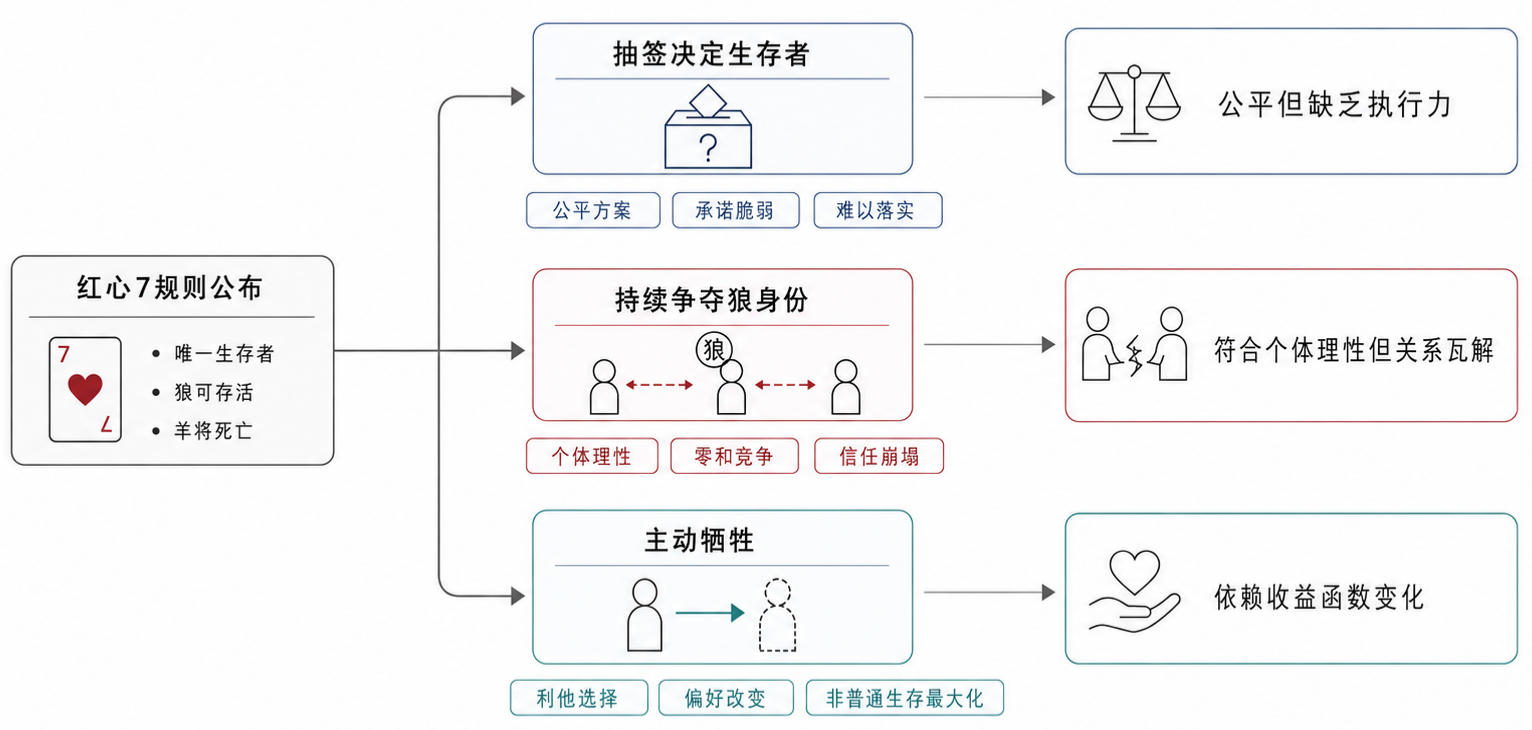
\includegraphics[width=1\textwidth]{fig/红心7的关键决策路径.png}
    \caption{红心7“狼与羊”的 if 线决策推演}
    \label{fig:heart7_if_tree}
\end{figure}

第一条路径是抽签决定最终生存者。这一方案看似能够降低内部冲突，因为它用随机机制替代直接争夺，也能在形式上满足公平原则。然而，抽签方案的问题在于无法自我执行。抽签失败者仍然可以在倒计时后期通过对视重新争夺狼身份。除非游戏额外提供强制装置，使抽签结果无法被推翻，否则该方案只是一种临时协调，而不是稳定均衡。

第二条路径是所有玩家共同合作并寻找规则漏洞。该方案体现了集体理性。如果玩家能够发现使所有人共同存活的方法，那么集体收益显然高于单人存活。然而，红心7的规则将最终生存条件明确绑定在狼身份上，且没有直接提供共同存活的信息。在缺乏确定漏洞的情况下，继续寻找规则漏洞会消耗时间，并增加玩家最终无法取得狼身份的风险。因此，这一方案在理论上代表集体最优想象，但在实际决策中面临信息不足和时间压力。

第三条路径是主动牺牲。与前两条路径相比，主动牺牲并不试图改变游戏规则，而是改变玩家自身的收益排序。牺牲者接受自身死亡，并将他人生存视为更高收益。该路径能够解释剧情中的情感强度，但它并不能被推广为所有玩家都会选择的稳定均衡。因为只有当玩家具有特定情感关系、道德偏好或心理动机时，牺牲才可能成为其可接受策略。对于一般玩家而言，主动牺牲仍然难以成为占优策略。

由此可见，红心7中的“没有别的选择”并不是指玩家没有行动空间，而是指许多看似可行的方案都无法同时满足生存、合作和稳定三个条件。抽签具有公平性但缺乏执行力，合作寻找漏洞具有集体理性但缺乏确定信息，主动牺牲具有情感意义但依赖特殊偏好。最终，红心7呈现出的不是单一人物的性格悲剧，而是零和规则、时间压力和承诺不可信共同作用下的结构性困境。

\subsection{红心7 小结}

红心7“狼与羊”的博弈结构可以概括为熟人关系被置入唯一生存名额规则后的非合作困境。游戏规则使玩家之间的收益关系接近零和，导致友情承诺难以稳定，口头协议缺乏执行力，抽签和轮流等方案也难以形成真正均衡。若玩家仅以自身生存为最高收益，争夺狼身份具有明显策略优势。若玩家最终选择牺牲，则说明其收益函数已经发生变化，友情、愧疚和道德意义被纳入收益判断之中。

因此，红心7的分析价值不在于简单说明人性自私或友情伟大，而在于揭示规则如何改变关系，收益结构如何压迫承诺，极端情境如何迫使玩家在个体理性与情感偏好之间重新排序。它为下一节分析红心J提供了基础。红心7中的核心资源是唯一生存名额，而红心J中的核心资源将转变为真实信息。前者展示信任如何被零和规则瓦解，后者则进一步展示信任如何在信息不对称中被建立、利用和破坏。

\section{红心J“单人牢房”的信息不对称与信任博弈分析}

\subsection{规则结构与信息不对称}

如果说红心7“狼与羊”的核心矛盾在于唯一生存名额所造成的零和竞争，那么红心J“单人牢房”的核心矛盾则在于信息不对称所造成的信任困境。在该游戏中，每名玩家项圈后方会显示一个花色，但玩家本人无法直接观察自己的花色，只能通过他人告知获得相关信息。每一轮结束时，玩家需要进入单人牢房并回答自己的花色，回答错误则会死亡。与此同时，玩家群体中隐藏着红心J。红心J并非普通的信息接收者，而是具有误导他人、破坏信任并维持自身隐藏状态的特殊玩家。

由此可见，红心J并不是一个单纯的记忆或猜测游戏。它的关键在于，玩家必须依赖他人才能获得自身生存所必需的信息，但又无法完全确认他人提供的信息是否真实。信息在这里不再只是辅助条件，而是决定生死的核心资源。玩家之间的互动也不再只是身体竞争或直接对抗，而是围绕“谁值得相信”“哪些信息可以验证”“谁可能是隐藏的红心J”展开的动态判断过程。

从博弈论角度看，红心J可以被理解为一个具有不完全信息特征的动态信任博弈。Akerlof\upcite{akerlof1970lemons}关于信息不对称的研究说明，当交易或互动双方掌握的信息不一致时，行为结果会受到信息差异的深刻影响。Harsanyi\upcite{harsanyi1967games}关于不完全信息博弈的研究进一步指出，玩家往往无法直接知道其他玩家的类型和真实意图，只能根据有限信息形成判断。红心J正是如此。普通玩家并不知道谁是红心J，也无法直接判断他人报出的花色是真是假，只能根据反复互动中的行为表现不断调整信念。

\begin{table}[H]
\centering
\caption{红心J“单人牢房”的玩家、策略与信息结构}
\label{tab:heartj_elements}
\renewcommand{\arraystretch}{1.35}
\begin{tabularx}{\textwidth}{C{3cm}Y}
\toprule
分析维度 & 内容说明 \\
\midrule
玩家 & 普通玩家与隐藏身份的红心J \\
核心规则 & 玩家无法看到自身花色，必须依赖他人提供信息 \\
普通玩家策略 & 如实告知、寻求他人告知、固定结盟、交叉验证、怀疑与排除 \\
红心J策略 & 隐藏身份、选择性提供真实信息、制造误导、破坏联盟、诱导错误回答 \\
核心收益 & 普通玩家需要回答正确并识别红心J，红心J需要隐藏身份并误导他人 \\
信息条件 & 玩家掌握他人花色信息，但无法直接观察自身花色，也无法确定他人类型 \\
博弈类型 & 不完全信息博弈、信号传递博弈、重复博弈 \\
主要矛盾 & 信任建立与信息操控之间的冲突 \\
\bottomrule
\end{tabularx}
\end{table}

表~\ref{tab:heartj_elements} 表明，红心J的复杂性来自双重信息不对称。第一重信息不对称存在于玩家自身花色和他人观察之间。玩家无法知道自己的花色，却必须依赖他人告知。第二重信息不对称存在于玩家身份和真实意图之间。普通玩家不知道谁是红心J，也不知道某个玩家提供信息时究竟是出于合作、试探还是误导。正是这两重信息不对称，使红心J中的信任关系具有高度不稳定性。

在这种规则结构下，玩家的理性策略不可能是简单地相信所有人，也不可能是完全拒绝他人信息。完全信任会使玩家容易被虚假信号操控，完全不信任则会使玩家无法获得回答自身花色所需的信息。因此，红心J中的核心策略问题不是“信任或不信任”这一简单二分，而是在不完全信息环境中如何建立有限信任、如何进行交叉验证，以及如何根据他人的行为持续更新判断。

\subsection{关键决策节点}

与红心7类似，红心J也可以被拆解为若干关键决策节点。不同之处在于，红心7的决策节点主要围绕生存名额展开，而红心J的决策节点主要围绕信息可信度展开。每一名玩家都必须在多个层面上作出判断，包括向谁询问花色，是否相信对方提供的信息，是否与某人固定结盟，是否公开共享信息，以及是否怀疑某人具有红心J身份。

\begin{table}[H]
\centering
\caption{红心J“单人牢房”的关键决策节点}
\label{tab:heartj_nodes}
\renewcommand{\arraystretch}{1.35}
\begin{tabularx}{\textwidth}{C{2.7cm}Y Y Y}
\toprule
决策节点 & 具体问题 & 可选策略 & 对应博弈概念 \\
\midrule
第一轮信息交换 & 玩家应当相信谁提供的花色 & 相信单一对象，询问多人，暂时观察 & 信息不对称，信号识别 \\
联盟形成阶段 & 玩家是否建立固定搭档关系 & 两两绑定，多人联盟，保持孤立 & 联盟博弈，重复博弈 \\
信任积累阶段 & 玩家如何判断对方是否可信 & 根据历史准确率判断，根据他人评价判断，交叉验证 & 声誉机制，贝叶斯更新 \\
怀疑出现阶段 & 玩家如何处理可疑信息 & 继续信任，降低信任，主动试探，公开质疑 & 信念更新，策略性怀疑 \\
红心J识别阶段 & 玩家如何锁定隐藏敌人 & 观察异常行为，比较信息矛盾，诱导暴露 & 不完全信息博弈，信号反制 \\
\bottomrule
\end{tabularx}
\end{table}

表~\ref{tab:heartj_nodes} 说明，红心J的博弈过程具有明显的动态性。玩家并不是在某一时刻一次性决定是否信任他人，而是在多轮互动中不断修正判断。某个玩家在前几轮提供正确信息，并不意味着其在后续回合一定继续可信。相反，隐藏身份的红心J可能通过前期合作建立声誉，再在关键节点释放错误信息，从而实现更有效的误导。由此可见，红心J中的信任并不是静态状态，而是一种不断被生产、检验和重估的策略资源。

\subsection{信号传递与信任建立}

红心J中的“报花色”行为可以被视为一种典型的信号传递。Spence\upcite{spence1973job}提出，信息较多的一方可以通过信号影响信息较少一方的判断。在红心J中，观察到他人花色的玩家拥有信息优势，而无法观察自身花色的玩家则处于信息劣势。前者通过语言告知后者花色，这一告知行为就是信号。若信号真实，接收者可以存活。若信号虚假，接收者可能死亡。

然而，信号能否被相信，并不只取决于信号内容本身，还取决于信号发送者的身份、动机和历史行为。普通玩家提供真实花色，可能是为了互相合作并延长生存时间。红心J提供真实花色，则可能是为了隐藏自己并积累可信声誉。红心J提供虚假花色，则可能是为了淘汰其他玩家并制造群体恐慌。因此，相同的“告知花色”行为，在不同玩家类型下具有不同含义。

\begin{figure}[H]
    \centering
    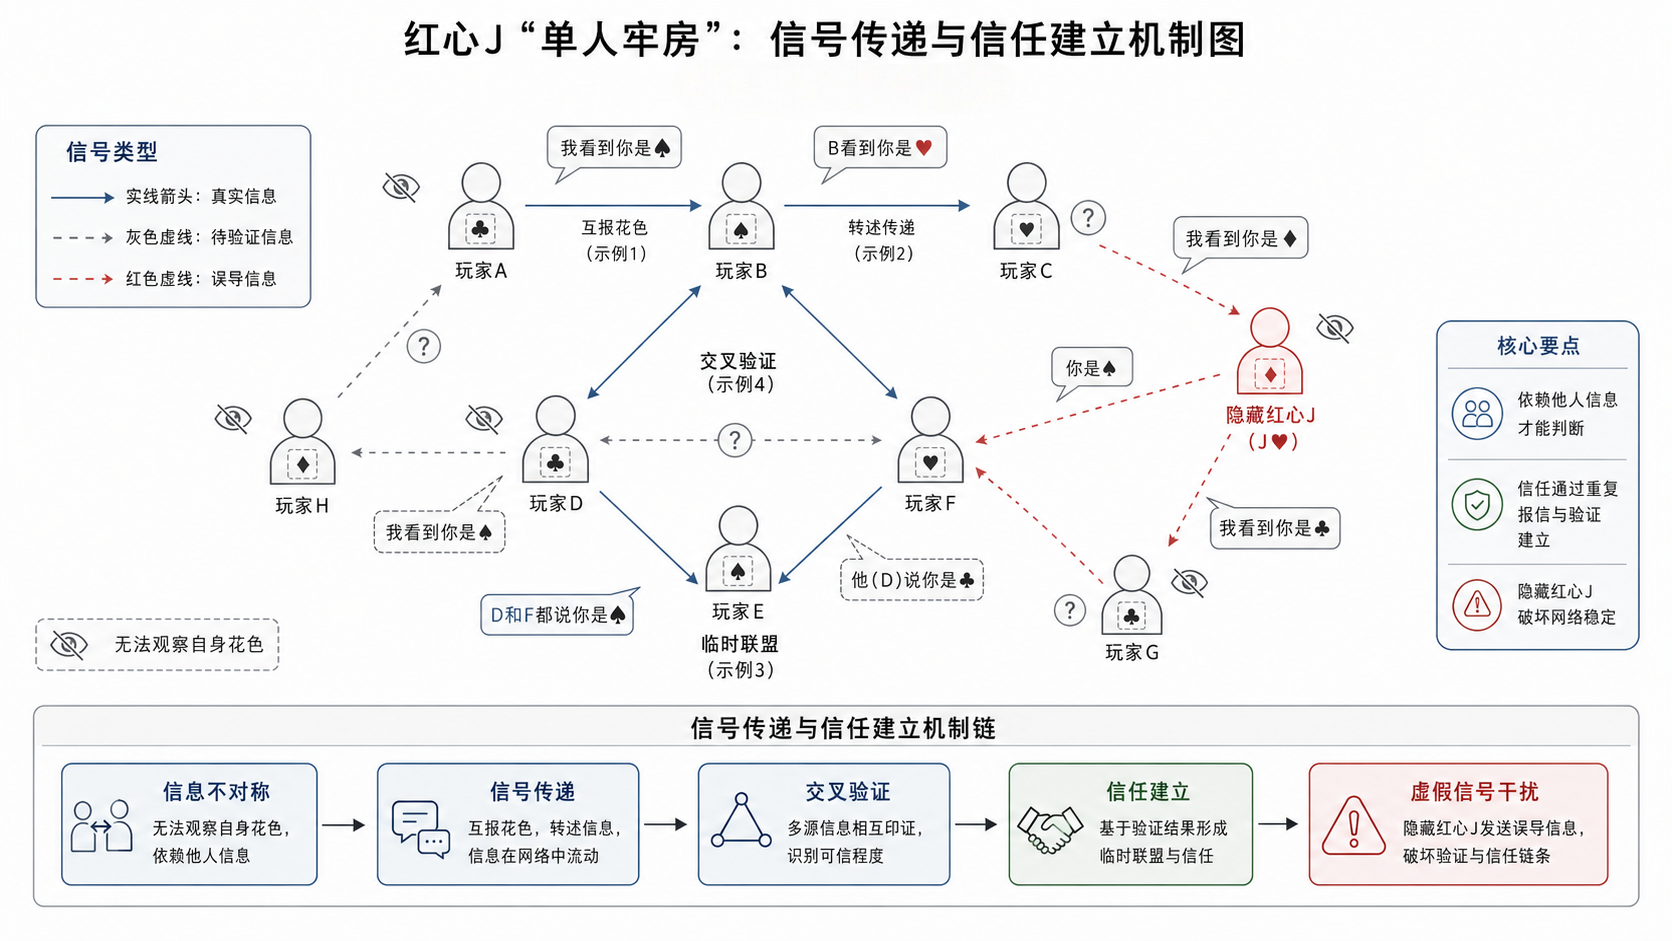
\includegraphics[width=1\textwidth]{fig/红心J单人牢房示意图.png}
    \caption{红心J“单人牢房”的信息传递与信任验证网络}
    \label{fig:heartj_signal_network}
\end{figure}

如图~\ref{fig:heartj_signal_network} 所示，红心J中的信息流并不是单向和透明的，而是由多个玩家之间的观察、告知、验证和怀疑共同构成。每名玩家既可能是信息发送者，也可能是信息接收者。玩家之间的关系也不是简单的朋友或敌人，而是随着每轮信息交换不断变化的信任网络。

在这一网络中，信任的建立通常依赖重复互动。如果某一玩家连续多轮提供正确信息，其可信度会提升，其他玩家也更愿意与其结盟。这体现了重复博弈中的声誉机制。声誉并不是玩家天然拥有的属性，而是在多轮行动中被逐步积累出来的结果。然而，红心J的存在使声誉机制变得复杂。隐藏敌人可以利用真实信号伪装成合作者，也可以利用局部合作换取长期信任。由此可见，声誉虽然能够降低不确定性，但并不能完全消除背叛风险。

\subsection{有限信任与交叉验证}

在红心J中，玩家面临三种基本信任策略。第一种是完全信任，即玩家依赖某个对象提供的信息，并直接根据该信息回答自己的花色。第二种是完全不信任，即玩家拒绝依赖他人信息，试图独立行动。第三种是有限信任与交叉验证，即玩家可以暂时接受某些信息，但会通过多名玩家、多个回合和行为一致性进行验证。

从策略效果看，完全信任的短期成本最低，因为玩家只需要依赖固定对象即可获得答案。如果对方确实可信，这种策略可以减少沟通成本并提高行动效率。但是，一旦对方是红心J，或者在关键时刻选择背叛，完全信任就会带来极高风险。完全不信任看似能够避免被欺骗，但由于玩家无法观察自身花色，这种策略实际上会使玩家失去生存所必需的信息来源。因此，完全不信任也不是稳定策略。

相较而言，有限信任与交叉验证更符合红心J的规则环境。玩家可以选择暂时相信某一信息源，但不将其视为唯一依据。通过询问多名玩家、比较不同信息是否一致、观察信息发送者的历史行为，玩家可以降低被单一虚假信号误导的概率。这一策略并不能彻底消除风险，但能在信息依赖和背叛防范之间取得相对平衡。

\begin{table}[H]
\centering
\caption{红心J中三种信任策略的比较}
\label{tab:heartj_trust_strategy}
\renewcommand{\arraystretch}{1.35}
\begin{tabularx}{\textwidth}{C{3cm}Y Y Y}
\toprule
策略类型 & 策略特征 & 主要优势 & 主要风险 \\
\midrule
完全信任 & 依赖单一对象提供花色信息 & 沟通成本低，行动效率高 & 容易被红心J或背叛者利用 \\
完全不信任 & 拒绝依赖他人信息，尽量独立判断 & 减少被单一对象操控的风险 & 无法获取自身花色，生存概率下降 \\
有限信任与交叉验证 & 暂时相信部分信息，同时通过多人和多轮验证 & 兼顾信息获取与风险控制 & 沟通成本较高，仍可能被多人合谋误导 \\
\bottomrule
\end{tabularx}
\end{table}

表~\ref{tab:heartj_trust_strategy} 表明，红心J的理性策略并不是绝对合作，也不是绝对孤立，而是在有限信任基础上的动态验证。这与红心7形成鲜明对比。红心7中，合作承诺之所以困难，是因为唯一生存名额使玩家之间的收益高度冲突。红心J中，合作之所以困难，则是因为信息真实性无法被立即确认。前者的问题是收益结构接近零和，后者的问题是信息结构高度不对称。

\subsection{红心J的得益结构与均衡分析}

为了进一步说明红心J中的信任困境，可以将其简化为两名普通玩家之间的信息互动。假设玩家A需要玩家B告知自己的花色。玩家A可以选择信任或验证，玩家B可以选择说真话或说假话。若玩家A信任且玩家B说真话，双方都能维持合作关系并获得生存收益。若玩家A信任而玩家B说假话，玩家A面临死亡风险，玩家B可能获得淘汰竞争者的收益。若玩家A选择验证，则可以降低被欺骗的风险，但需要承担沟通成本。若玩家B说假话而玩家A进行验证，玩家A可能识别出异常，玩家B的可信度下降。

\begin{table}[H]
\centering
\caption{红心J中信息告知与信任选择的简化得益矩阵}
\label{tab:heartj_payoff}
\renewcommand{\arraystretch}{1.4}
\begin{tabular}{C{3.5cm}C{4cm}C{4cm}}
\toprule
 & 玩家B说真话 & 玩家B说假话 \\
\midrule
玩家A直接信任 & $(5,5)$ & $(-10,8)$ \\
玩家A交叉验证 & $(3,4)$ & $(2,-3)$ \\
\bottomrule
\end{tabular}
\end{table}

表~\ref{tab:heartj_payoff} 中的数值同样是相对收益，用于表达策略结果的差异。直接信任在对方诚实时收益最高，因为双方都能以较低成本维持合作。但当对方说假话时，直接信任会使玩家A承受极大损失。交叉验证虽然降低了合作效率，却能在对方说假话时减少损失，并可能使欺骗者承担声誉下降或身份暴露的代价。

从均衡角度看，红心J难以形成“所有人完全信任”的稳定状态。只要群体中存在隐藏的红心J，虚假信号就始终具有策略价值。对于红心J而言，在关键时刻误导他人可以直接减少竞争者并制造混乱。因此，完全信任容易被破坏。另一方面，所有人完全不信任也不是稳定状态，因为玩家无法独立观察自己的花色，若拒绝一切信息交换，就无法完成每轮回答。因此，红心J更可能形成一种介于信任和怀疑之间的动态均衡。玩家需要进行信息交换，但同时保留验证机制和怀疑空间。

这种均衡可以概括为“有限信任均衡”。在该状态下，玩家不会无条件相信任何单一对象，也不会完全拒绝合作。玩家会根据历史行为、他人反馈和信息一致性判断某一信号的可信度。若某人多轮提供正确信息，其可信度上升。若某人信息前后矛盾，或其提供的信息与其他人的观察不一致，其可信度下降。由此，信任在红心J中成为一种可积累、可消耗、也可被操控的资源。

\subsection{红心J if 线推演}

红心J同样适合进行 if 线推演。通过比较不同策略路径，可以更清楚地看到为什么有限信任和交叉验证比完全信任或完全孤立更接近理性选择。本文可以设置三条主要推演路径，分别是全员公开互报花色、两两固定绑定以及多人交叉验证。

第一条路径是全员公开互报花色。该方案表面上最接近集体合作。如果所有玩家都如实公开他人花色，那么普通玩家可以最大限度地降低死亡风险，并通过长期观察找出可疑者。然而，该方案的关键问题在于红心J也参与其中。红心J可以在前期提供真实信息以维持身份隐藏，再在关键时刻制造一次虚假信息，诱导某名玩家回答错误。由于全员公开依赖群体诚实，一旦隐藏敌人能够策略性说谎，完全公开就无法保证稳定。

第二条路径是两两固定绑定。该方案通过缩小信任范围降低沟通成本。玩家只需要依赖固定搭档告知花色，双方可以通过重复互动建立较强关系。与全员公开相比，两两绑定更容易形成稳定声誉，也更便于判断搭档是否异常。然而，它的风险在于，一旦搭档本身就是红心J，或者搭档被他人误导，玩家就会高度依赖单一信息源，缺乏纠错空间。因此，两两绑定能够提高局部信任，却也会带来信息来源过窄的问题。

第三条路径是多人交叉验证。该方案要求玩家从多个来源确认自身花色，并比较不同信息之间是否一致。它的优势在于可以降低单一虚假信号带来的风险，也能够通过信息矛盾发现潜在欺骗者。其缺点是沟通成本较高，并且在群体混乱或多人合谋时仍可能失败。不过，在存在隐藏敌人的条件下，多人交叉验证比完全信任和单一绑定更具稳健性。它不是收益最高的理想策略，却是风险控制能力更强的现实策略。


\begin{figure}[H]
    \centering
    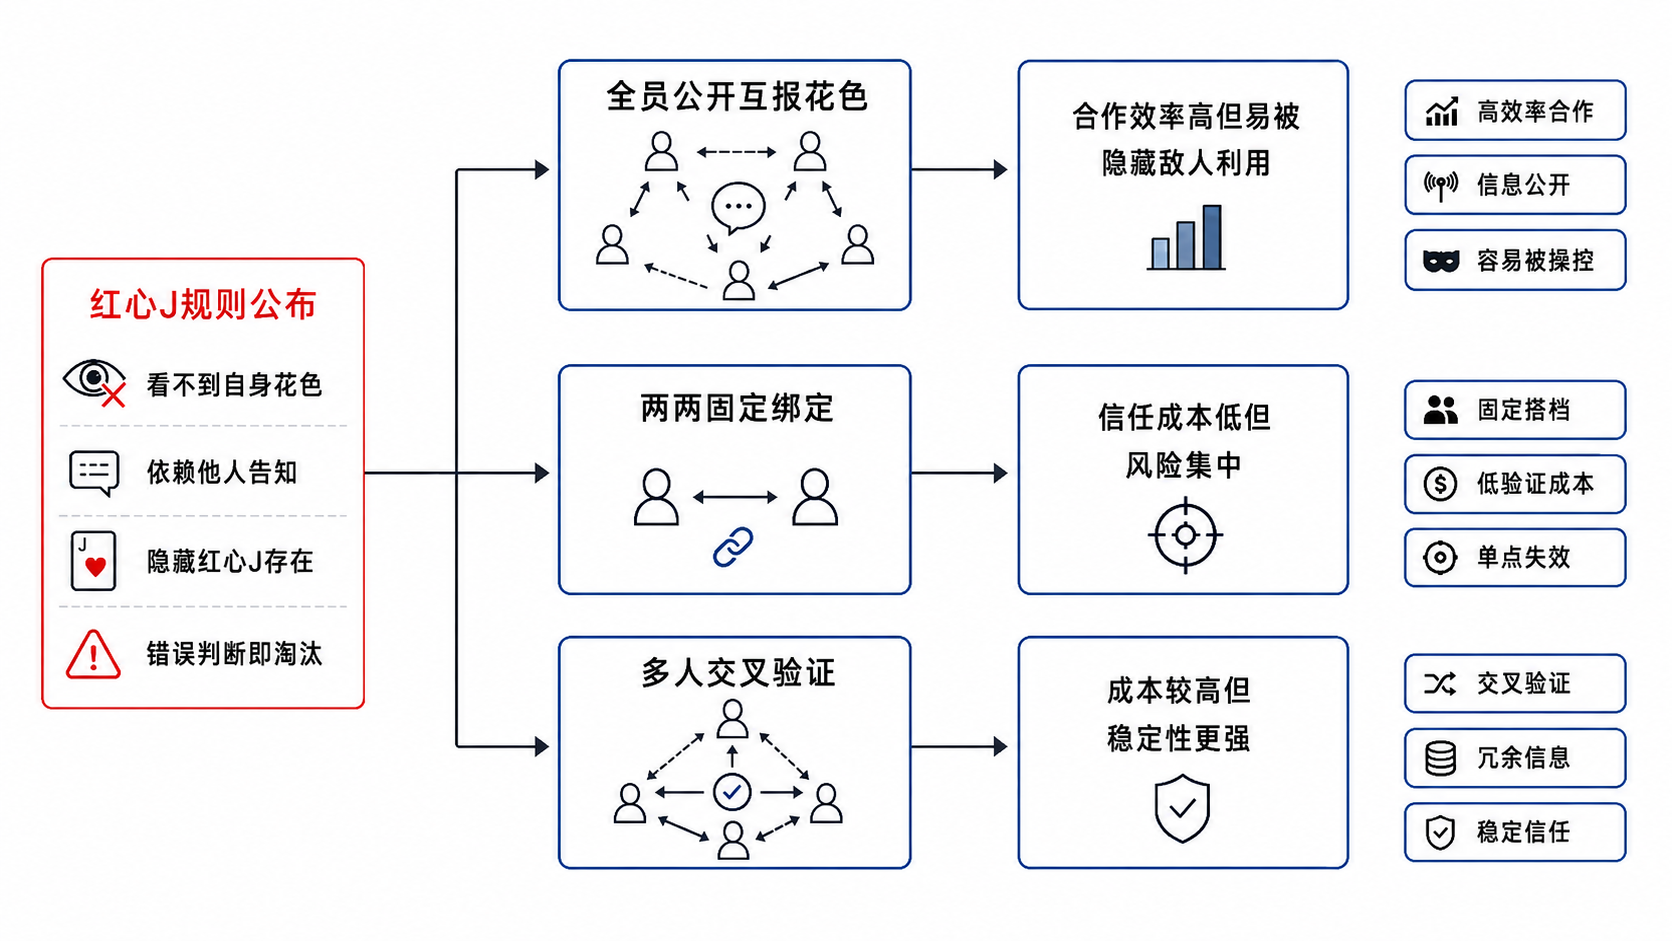
\includegraphics[width=1\textwidth]{fig/红心Jif线情况分析.png}
    \caption{红心J“单人牢房”的 if 线决策推演}
    \label{fig:heartj_if_tree}
\end{figure}

通过上述推演可以看出，红心J中的策略选择并不存在绝对安全的方案。全员公开依赖所有人诚实，但红心J的存在破坏了这一前提。两两绑定能够降低信任成本，却会扩大单一搭档背叛带来的损失。多人交叉验证提高了判断稳健性，却增加了时间和沟通成本。因此，红心J呈现的并不是简单的“相信别人会死”或“不相信别人才能活”，而是一个更复杂的信任权衡过程。玩家必须在信息依赖、验证成本和背叛风险之间不断寻找相对稳定的策略。

\subsection{小结}

红心J“单人牢房”的博弈结构可以概括为信息不对称条件下的动态信任博弈。玩家无法观察自身花色，却必须依赖他人提供信息。隐藏的红心J则利用这一信息结构进行误导、伪装和破坏。与红心7中围绕唯一生存名额展开的零和竞争不同，红心J的核心资源是真实信息，核心矛盾是信任建立与信息操控之间的冲突。

红心J的分析说明，在不完全信息环境中，信任并不是天然稳定的关系，而是一种需要通过多轮信号、声誉和验证机制逐步建立的策略资源。完全信任容易被隐藏敌人利用，完全不信任又无法获得必要信息。相对合理的策略是有限信任与交叉验证，即在接受信息的同时保持怀疑，并通过多人、多轮和多渠道确认降低被误导的风险。由此，红心J将红心7中的“信任被规则瓦解”进一步推进为“信任被信息生产、利用和破坏”的过程，也为下一部分比较两个红心游戏的理论递进关系奠定基础。

\section{两种红心游戏的比较与理论递进}

\subsection{从生存名额竞争到真实信息竞争}

通过前文分析可以看出，红心7与红心J虽然都属于红心类型游戏，但二者所呈现的博弈结构并不相同。红心7的核心资源是唯一生存名额，玩家的主要目标是争夺最终的狼身份。红心J的核心资源则是真实信息，玩家的主要目标是获得关于自身花色的可靠判断，并识别隐藏在群体中的红心J。前者的冲突来自规则直接制造的生存排他性，后者的冲突来自信息不对称造成的信任不确定性。

这种差异使两个游戏在理论上形成了递进关系。红心7更接近零和生存博弈，它展示的是当生存资格只能由一人获得时，熟人之间的友情承诺为什么难以维持。红心J则更接近不完全信息条件下的动态信任博弈，它展示的是当玩家必须依赖他人提供信息时，信任如何被建立、检验、操控和破坏。二者共同说明，红心游戏的残酷性并不只是来自死亡惩罚，而是来自规则与信息对玩家关系的重构。

\begin{table}[H]
\centering
\caption{红心7与红心J的博弈结构比较}
\label{tab:heart_compare}
\renewcommand{\arraystretch}{1.35}
\begin{tabularx}{\textwidth}{C{3cm}Y Y}
\toprule
比较维度 & 红心7“狼与羊” & 红心J“单人牢房” \\
\midrule
核心资源 & 唯一生存名额 & 真实花色信息 \\
玩家关系 & 熟人关系，原本存在友情和情感纽带 & 陌生人关系，依靠临时联盟建立信任 \\
基本规则 & 最终只有狼能够存活，羊会死亡 & 玩家无法看到自身花色，必须依赖他人告知 \\
主要矛盾 & 生存竞争与友情承诺之间的冲突 & 信任建立与信息操控之间的冲突 \\
信息结构 & 规则相对明确，结果高度零和 & 信息不对称，身份与意图难以判断 \\
主要策略 & 争夺狼身份，逃避对视，承诺让渡，主动牺牲 & 如实告知，虚假告知，固定结盟，交叉验证 \\
对应理论 & 零和博弈，非合作博弈，承诺可信性，纳什均衡 & 不完全信息博弈，信号传递，重复博弈，贝叶斯更新 \\
均衡困境 & 合作承诺难以稳定，失败者存在偏离动机 & 完全信任容易被利用，完全不信任无法生存 \\
理论意义 & 说明规则如何瓦解熟人信任 & 说明信息如何生产并破坏陌生人信任 \\
\bottomrule
\end{tabularx}
\end{table}

表~\ref{tab:heart_compare} 表明，两个游戏虽然都围绕信任展开，但信任失效的原因并不相同。红心7中，信任失效主要源于收益结构。只要最终只能有一人存活，合作承诺就会受到死亡风险的持续冲击。红心J中，信任失效主要源于信息结构。即使玩家具有合作意愿，也无法确认他人是否真实、稳定、无害地提供信息。因此，红心7中的信任困境更接近“利益冲突下的承诺不可信”，红心J中的信任困境更接近“信息不对称下的信号不可信”。

\subsection{规则如何改变收益结构}

博弈论分析强调，玩家的行动不能脱离规则与收益结构来理解。Osborne 和 Rubinstein\upcite{osborne1994course}关于博弈结构的基本讨论说明，玩家、策略和收益共同决定了互动结果。将这一思路应用到红心游戏中可以发现，人物行为并不是单纯由性格决定的，而是在特定规则下被重新塑造的。

在红心7中，游戏规则将玩家置于唯一生存名额的竞争中。即便玩家之间原本存在友情，规则仍然使得生存收益与他人死亡结果高度绑定。正因如此，抽签、轮流和口头承诺等方案虽然具有道德吸引力，却缺少稳定的执行基础。玩家不是不知道合作更温和，而是因为合作结果无法被规则保障。只要某一玩家在最后阶段仍然能够通过对视改变狼身份，那么该玩家就始终具有偏离协议的可能。

红心J的规则对收益结构的改变方式则不同。它并不直接规定只有一名普通玩家能够存活，而是让每名玩家都必须依赖他人信息才能活下去。这样一来，玩家的收益不仅取决于自身判断能力，也取决于他人是否愿意提供真实信息。信息发送者因而获得策略优势。普通玩家可以通过真实信号建立信任，红心J也可以通过真假混合的信号操控他人。由此，信息本身成为一种可以影响收益分配的资源。

因此，红心7和红心J都说明了一个共同问题。死亡游戏中的人物选择并不是在抽象道德空间中发生的，而是在规则塑造出的收益空间中发生的。规则不是背景，而是决定玩家关系的核心机制。规则一旦改变，友情、合作、信任和背叛的含义也会随之改变。

\subsection{信任机制的两种瓦解方式}

红心7与红心J也可以被理解为信任机制的两种瓦解方式。红心7展示的是信任被零和规则瓦解。玩家之间即使愿意相信彼此，也无法消除唯一生存名额带来的根本冲突。信任在这里面临的是收益层面的压力。只要一方生存意味着另一方死亡，信任就难以成为稳定策略。换言之，红心7中的问题不是玩家无法交流，而是交流无法改变零和收益结构。

红心J展示的则是信任被信息不对称瓦解。玩家之间必须交流，也必须在一定程度上依赖他人。问题在于，交流本身可能被操控。某个玩家说出的花色可能是真实信息，也可能是红心J释放的误导信号。信任在这里面临的是信息层面的压力。玩家不是没有合作需求，而是无法确认合作对象的真实身份与真实意图。

这两种瓦解方式对应两种不同的博弈困境。红心7中的困境是“我是否愿意牺牲自己的收益来成全他人”。红心J中的困境是“我是否能够判断他人的信息是否可信”。前者强调收益冲突，后者强调信念不确定。前者导致承诺不稳定，后者导致信号不稳定。由此，两个游戏在理论上不是简单并列，而是从收益冲突推进到信息冲突，从熟人关系推进到陌生人社会，从个体生存推进到群体信任。

\subsection{从非合作到有限合作}

红心7和红心J都不是简单否定合作可能性的游戏。相反，它们都说明合作可以出现，但合作必须受到规则、信息和执行条件的限制。红心7中，合作之所以困难，是因为缺乏能够约束偏离行为的机制。玩家即便达成协议，也无法保证协议在最后阶段被遵守。红心J中，合作之所以困难，是因为玩家无法确认合作对象是否真实可信。即便某个玩家连续提供正确信息，也可能只是隐藏敌人积累声誉的策略。

因此，两个游戏都指向一种有限合作的逻辑。红心7中的合作只有在玩家收益函数发生变化时才可能稳定，例如牺牲者将朋友生存视为高于自身生存的价值。红心J中的合作只有在验证机制存在时才更可靠，例如玩家通过多人交叉确认和多轮观察降低虚假信号风险。前者说明合作需要偏好基础，后者说明合作需要信息基础。

这一点可以回应本文开头提出的问题。关键人物为什么没有选择其他路径，并不是因为他们完全没有选择，而是因为多数路径缺乏稳定条件。红心7中，抽签和轮流缺少执行机制。红心J中，全员公开和两两绑定都可能被隐藏敌人利用。角色看似可以选择合作、隐瞒、背叛或牺牲，但这些选择能否成为稳定结果，取决于收益结构是否支持，信息条件是否允许，偏离行为是否能够被约束。

\subsection{理论递进与研究框架总结}

综合前文，本文可以将红心7与红心J的递进关系概括为三层。第一层是玩家关系的递进。红心7发生在熟人关系中，红心J发生在陌生人关系中。第二层是核心资源的递进。红心7争夺的是唯一生存名额，红心J争夺的是可靠信息。第三层是理论问题的递进。红心7强调零和规则如何破坏承诺，红心J强调信息不对称如何重塑信任。

% 这里建议加入一张总结图
% 图名建议为 heart_games_framework.png
% 放置位置建议在本段之后
% 图中可以画出一条横向递进链条
% 红心7 零和生存博弈
% 箭头指向 红心J 信息信任博弈
% 再箭头指向 本文核心命题
% 规则改变收益结构，信息改变信任机制

\begin{figure}[H]
    \centering
    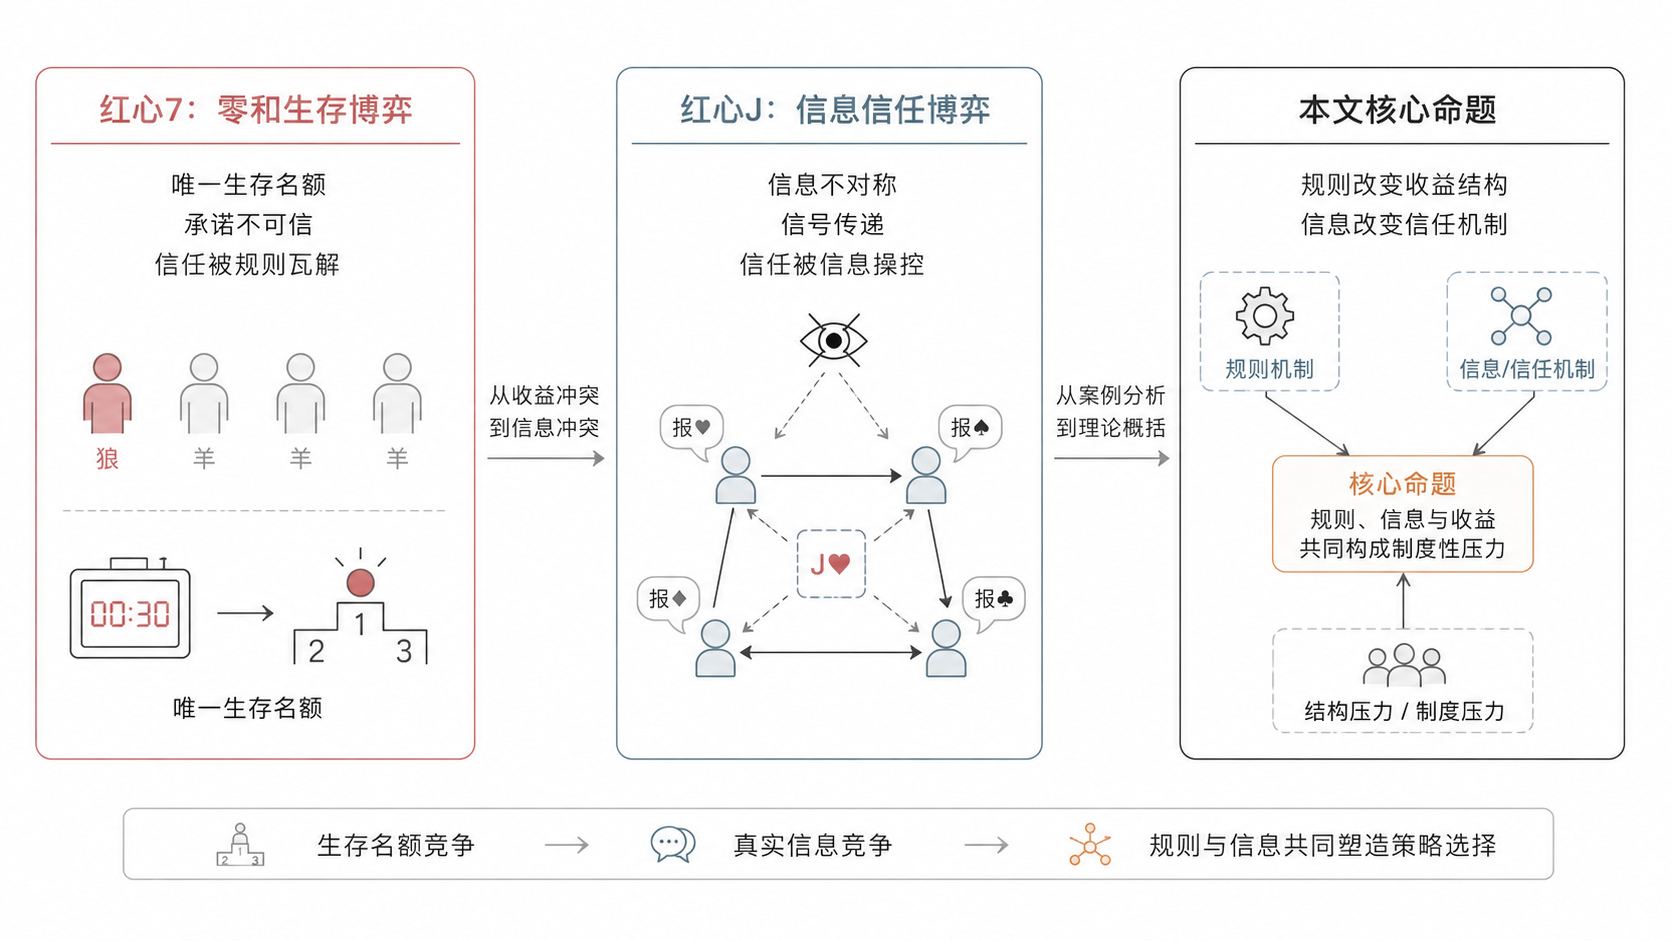
\includegraphics[width=1\textwidth]{fig/红心游戏.png}
    \caption{红心7与红心J的理论递进关系}
    \label{fig:heart_games_framework}
\end{figure}

如图~\ref{fig:heart_games_framework} 所示，红心7和红心J共同构成了从“零和生存博弈”到“信息信任博弈”的递进链条。红心7说明，规则可以通过改变收益结构瓦解熟人之间的信任。红心J说明，信息可以通过改变判断条件重塑陌生人之间的信任。两者共同指向本文的核心命题。死亡游戏中的残酷并不只来自惩罚，而来自规则、信息和收益共同构成的制度性压力。

这一递进关系也使本文区别于一般剧情解读。一般剧情解读往往关注人物是否善良、是否背叛、是否牺牲。本文则关注这些行为背后的结构性原因。也就是说，本文并不简单评价人物选择，而是分析这些选择在何种规则下成为合理策略，在何种信息条件下失去稳定性，又在何种偏好变化下发生转向。通过这种方式，《弥留之国的爱丽丝》中的红心游戏可以被理解为非合作博弈与信任机制的叙事化呈现。

\subsection{小结}

本节从比较角度说明了红心7与红心J之间的理论递进关系。红心7以唯一生存名额为核心，呈现了零和规则下熟人信任的瓦解。红心J以真实信息为核心，呈现了信息不对称下陌生人信任的建立、利用和破坏。前者强调收益冲突，后者强调信息不确定。前者说明合作承诺为什么不可信，后者说明信号传递为什么需要验证。

由此可以得出，两个红心游戏并不是两个彼此独立的案例，而是共同构成了一条从生存竞争到信任治理的分析链条。红心7回答的是在唯一生存资格面前，友情为什么难以维持。红心J回答的是在信息无法完全确认时，信任为什么必须被验证。二者结合，使本文能够从规则、收益、信息和均衡四个层面解释死亡游戏中的人物选择。

\section{讨论：死亡游戏中的理性选择与均衡边界}

\subsection{人物是否真的“没有别的选择”}

通过前文对红心7和红心J的分析可以发现，死亡游戏中的人物并非完全没有行动选项。相反，他们在每一个关键节点上都面对多种可能策略。红心7中的玩家可以选择争夺狼身份、接受抽签、继续合作、逃避对视或主动牺牲。红心J中的玩家也可以选择完全信任、完全不信任、两两绑定、公开互报或多人交叉验证。由此可见，所谓“没有别的选择”并不是指玩家在行动层面没有可选方案，而是指多数方案在既定规则和信息条件下难以形成稳定结果。

从博弈论角度看，策略是否可行，不能只看它在道德上是否合理，也不能只看它在剧情上是否令人期待，而要看它是否具有稳定性。红心7中的抽签方案看似公平，但无法阻止失败者在最后阶段重新争夺狼身份。红心J中的全员公开方案看似高效，但无法排除隐藏红心J策略性说谎的可能。也就是说，许多“看起来更好”的选择并不是不存在，而是缺少成为均衡的条件。

因此，本文所说的均衡并不是指人物必然作出了最优选择，而是指在特定规则下，某些选择会受到结构性压力的限制。人物可能知道还有其他方案，但这些方案要么缺少执行机制，要么面临信息不足，要么依赖特殊的情感偏好。红心游戏的残酷性正体现在这里。它并不只是剥夺玩家的生命，也通过规则设计压缩了稳定合作的空间。

\subsection{个体理性与集体理性的冲突}

红心7最集中地体现了个体理性与集体理性的冲突。若从集体角度看，玩家之间保持合作、减少冲突和尝试寻找规则漏洞，显然比互相追逐和互相怀疑更符合整体利益。但从个体角度看，最终只有狼能够存活，任何处于羊身份的玩家都无法忽视自身死亡风险。在这种情况下，个体理性会不断侵蚀集体合作的基础。

这一问题与囚徒困境具有一定相似性。囚徒困境说明，在缺乏有效约束和可信承诺的情况下，个体追求自身较优结果可能导致集体结果恶化。红心7虽然不是标准囚徒困境，因为其规则更接近唯一生存者的零和结构，但它同样揭示了合作难以维持的原因。玩家并非不知道合作具有情感价值，而是无法确认他人会不会在最后阶段偏离合作。

红心J中的个体理性与集体理性冲突则更加隐蔽。对普通玩家而言，互相提供真实信息有助于延长整体生存时间，也有助于逐渐锁定红心J。然而，个体玩家仍然可能隐瞒信息、选择性告知或只保护自己的联盟对象。对于红心J而言，破坏集体信任则符合自身利益。因此，即使普通玩家之间存在合作需求，整体合作也会受到隐藏敌人的持续干扰。

这说明，死亡游戏中的集体理性往往需要三个条件。第一，玩家之间的收益不能完全对立。第二，合作承诺需要某种执行或验证机制。第三，玩家需要具备足够的信息来判断他人是否遵守合作。红心7缺少第一个条件，红心J缺少第三个条件。正因如此，两个游戏都难以形成稳定的全面合作。

\subsection{均衡边界与非标准收益}

前文分析表明，如果将生存设定为唯一收益，红心7中的争夺狼身份会具有很强的策略吸引力，红心J中的交叉验证也会比单纯信任更加稳健。然而，影视叙事中的人物并不是只有单一收益目标。友情、愧疚、尊严、道德责任和自我认同都会影响人物的选择。也正因为如此，本文在使用博弈论模型时，需要承认模型解释的边界。

红心7中的牺牲行为就是一个典型例子。如果按照狭义自利理性，主动牺牲并不是生存收益最大化的选择。但如果将朋友存活、关系意义和道德完整性纳入收益函数，牺牲行为就不再是完全非理性的。它不是规则结构直接导出的均衡，而是人物在极端压力下重塑收益排序后的结果。换言之，牺牲行为突破了标准生存收益模型，但并没有完全脱离策略解释。

红心J中也存在类似情况。玩家之间的信任并不总是经过严格计算后形成。某些信任可能来自直觉、情感依赖或临时共同体意识。但在死亡风险和隐藏敌人同时存在的条件下，这些信任如果缺乏验证机制，就容易被转化为策略漏洞。因此，红心J并不是否定信任，而是说明信任必须被制度化为可观察、可验证和可修正的互动过程。

由此可见，博弈论能够解释红心游戏中的许多结构性选择，但不能完全取代人物心理和叙事意义。本文的模型化分析并不是要把人物简化为冷冰冰的收益机器，而是要说明在极端规则下，人物情感如何被收益结构压迫，又如何在某些时刻改变收益结构本身。

\subsection{if 线推演的理论意义}

本文在分析红心7和红心J时都加入了 if 线推演。其目的并不是进行剧情改写，而是通过反事实路径检验不同策略是否具备稳定条件。若某一策略在想象中看似更好，但在规则限制下无法防止偏离行为或无法解决信息不对称问题，那么它就难以成为真正可持续的选择。

红心7中的 if 线说明，抽签、轮流和寻找漏洞等方案虽然具有一定合理性，但都面临执行问题。只要玩家仍然可以通过对视转移狼身份，任何协议都可能在倒计时末期失效。主动牺牲能够带来稳定结果，但它依赖特殊偏好，不能被视为一般玩家都会接受的均衡策略。

红心J中的 if 线则说明，全员公开、两两绑定和多人交叉验证各有优劣。全员公开在所有人诚实的前提下效率最高，但隐藏红心J的存在破坏了这一前提。两两绑定降低了信任成本，但会造成风险集中。多人交叉验证虽然成本较高，却更能抵抗单一虚假信号。因此，红心J中的理性策略更接近有限信任，而不是绝对信任或绝对怀疑。

\begin{table}[H]
\centering
\caption{红心7与红心J中 if 线方案的稳定性比较}
\label{tab:if_stability}
\renewcommand{\arraystretch}{1.35}
\begin{tabularx}{\textwidth}{C{3cm}Y Y Y}
\toprule
游戏 & if 线方案 & 表面优势 & 稳定性问题 \\
\midrule
红心7 & 抽签决定生存者 & 形式公平，减少直接冲突 & 缺少执行机制，失败者仍可偏离 \\
红心7 & 共同寻找规则漏洞 & 符合集体理性，可能实现共同存活 & 信息不足，时间压力大，成功不确定 \\
红心7 & 主动牺牲 & 能形成明确结果，保全他人 & 依赖特殊偏好，难以普遍化 \\
红心J & 全员公开互报花色 & 合作效率高，信息流通充分 & 隐藏红心J可策略性说谎 \\
红心J & 两两固定绑定 & 信任成本低，重复互动稳定 & 风险集中，搭档若不可信则损失极大 \\
红心J & 多人交叉验证 & 抗欺骗能力较强，信息更稳健 & 沟通成本高，仍可能被复杂误导影响 \\
\bottomrule
\end{tabularx}
\end{table}

表~\ref{tab:if_stability} 说明，if 线推演能够帮助本文避免停留在“人物为什么不这样做”的直觉质疑上。许多替代方案并非没有被想到，而是在更严格的博弈条件下缺乏稳定性。通过比较不同路径的收益、风险和执行条件，可以更清楚地解释人物选择的结构性限制。

\subsection{小结}

本节从理性选择、集体合作、均衡边界和 if 线推演四个方面，对前文案例分析进行了进一步讨论。红心7和红心J共同说明，人物并不是没有选择，而是在特定规则和信息条件下，许多选择无法形成稳定均衡。红心7中的困境来自零和收益结构，红心J中的困境来自信息不对称。前者使合作承诺难以执行，后者使信任关系必须接受验证。

与此同时，本文也承认博弈论模型存在解释边界。死亡游戏中的人物不仅追求生存，也会受到友情、愧疚和道德意义的影响。正因为如此，红心游戏的分析不能只停留在冷静的收益计算，也需要理解人物如何在极端规则下重新排序自己的价值。博弈论在这里提供的不是对人性的替代解释，而是对剧情冲突背后规则结构的揭示。

\section{结论}

本文以《弥留之国的爱丽丝》中的红心7“狼与羊”和红心J“单人牢房”为研究对象，尝试从博弈论视角分析死亡游戏中的非合作行为与信任机制。与单纯的剧情解读不同，本文并未将人物行为简单归结为善良、自私、背叛或牺牲，而是从游戏规则出发，将人物转换为玩家，将行为转换为策略，将剧情冲突转换为收益结构和信息结构，并通过得益矩阵、关键决策节点和 if 线推演解释人物选择背后的结构性原因。

研究发现，红心7的核心矛盾在于唯一生存名额所造成的零和竞争。游戏规则规定最终只有狼能够存活，这使得玩家之间原本存在的友情关系被重新嵌入生存竞争之中。在这一结构下，抽签、轮流和口头承诺等方案虽然具有道德吸引力，却难以形成稳定均衡。原因在于这些方案缺乏外部执行机制，且失败者在死亡压力下始终存在偏离协议的动机。因此，红心7所呈现的并不是简单的人性崩塌，而是零和规则对熟人信任的制度性瓦解。

与红心7相比，红心J的核心矛盾并不在于唯一生存名额，而在于信息不对称。玩家无法看到自己的花色，只能依赖他人提供信息。与此同时，隐藏身份的红心J具有操控信息、误导他人和破坏信任的动机。因此，红心J中的信任并不是天然稳定的关系，而是一种需要通过多轮信号、声誉积累和交叉验证不断生产和检验的策略资源。完全信任容易被隐藏敌人利用，完全不信任又会使玩家失去必要信息。相对而言，有限信任与交叉验证更接近该游戏中的稳健策略。

通过比较可以看出，红心7与红心J之间形成了清晰的理论递进。红心7展示的是“生存名额竞争”如何瓦解熟人之间的承诺与信任，红心J则进一步展示“真实信息竞争”如何重塑陌生人之间的合作与怀疑。前者强调收益结构对玩家关系的压迫，后者强调信息结构对信任机制的改造。二者共同说明，红心游戏的残酷性并不只来自死亡惩罚，而来自规则、收益与信息共同构成的制度环境。人物看似拥有多种选择，但许多选择在既定规则下缺乏稳定条件，因而难以成为真正可持续的策略。

本文的分析也表明，所谓“人物没有别的选择”并不意味着人物没有行动空间，而是指许多替代方案无法同时满足生存、合作和稳定三个条件。红心7中的抽签方案缺少执行力，红心J中的全员公开方案容易被隐藏敌人利用。角色之所以没有选择某些看似更好的路径，并非完全出于情绪或偶然，而是因为这些路径在博弈结构中存在偏离动机、信息缺口或验证成本。通过 if 线推演，本文进一步说明了反事实路径的意义在于检验策略的稳定性，而不是简单改写剧情。

当然，本文也存在一定局限。由于研究对象是影视文本，剧情本身包含情感表达、人物成长和戏剧化安排，不能被完全还原为标准博弈模型。得益矩阵中的数值也只是对相对收益关系的抽象表达，并不代表角色真实心理收益的精确测量。因此，本文的模型化分析更适合被理解为一种解释框架，而不是严格形式化证明。后续研究可以进一步引入更多红心游戏，或比较黑桃、方块、梅花等不同类型游戏的博弈结构，从而更系统地分析《弥留之国的爱丽丝》中规则设计与人物行为之间的关系。

总体而言，《弥留之国的爱丽丝》中的红心游戏为理解非合作博弈与信任机制提供了具有代表性的叙事场景。红心7说明，规则可以通过改变收益结构摧毁熟人关系中的合作基础。红心J说明，信息可以通过改变判断条件影响陌生人之间的信任形成。二者共同揭示了一个核心命题，即在极端制度环境下，人的选择并不只是道德品质的体现，也是在规则、信息和收益压力下形成的策略结果。正是在这一意义上，红心7与红心J不仅是具有戏剧张力的死亡游戏，也可以被视为分析理性选择、信任边界和均衡条件的博弈论案例。

\bibliographystyle{gbt7714-numerical}
\bibliography{sample}

\end{document}